% Chapter Template

\chapter{Estado del Arte} % Main chapter title

\label{Chapter2} % Change X to a consecutive number; for referencing this chapter elsewhere, use \ref{ChapterX}

%----------------------------------------------------------------------------------------
%	SECTION 1
%----------------------------------------------------------------------------------------

\section{An\'alisis  de im\'agenes de la retina}

En esta Secc\'in describiremos en detalle.... En la Secci\'on

	\subsection{Introducci\'on}


La retinopat\'ia diab\'etica (RD) es el l\'ider en las patolog\'ias oftalmol\'ogicas y causante de ceguera entre las personas en edad de trabajar en los pa\'ises desarrollados . Est\'a provocada por complicaciones en la diabetes mellitus y , aunque los efectos de la diabetes no necesariamente implican el deterioro de la visión , el 2\% de los pacientes afectados por este trastorno son ciegos y el 10\% padecen  degradaci\'on de la visi\'on despu\'es de 15 años de diabetes como consecuencia de complicaciones RD . La prevalencia estimada de diabetes por todos los grupos de edad en todo el mundo fue de 2,8\% en 2000 y 4,4\% en 2030 , lo que significa que el n\'umero total de pacientes con diabetes se prev\'e aumente de 171 millones en el  2000 a 366 millones en el 2030 .
	A pesar de que la RD es una enfermedad incurable, la fotocoagulaci\'on l\'aser puede prevenir la p\'erdida de la visi\'on si es detectada en etapas tempranas. Sin embargo, los pacientes con RD no perciben ning\'un s\'intoma hasta que la p\'erdida de visi\'on se desarrolla, por lo general en estadios de la enfermedad más adelantados, cuando el tratamiento es menos eficaz. Entonces, para garantizar que el tratamiento es recibido a tiempo, los pacientes diab\'eticos necesitan un examen anual de fondo de ojo. Sin embargo, esta acci\'on preventiva involucra presenta un enorme desaf\'io para el Sistema de Salud debido  al gran n\'umero de pacientes que necesitan revisi\'on oftalmológica. Por lo tanto, la RD tambi\'en llega a ser un gran problema econ\'omico en la  Administraci\'on P\'ublica ya que ,solo en U.S, el costo de las complicaciones oftalmol\'ogicas cr\'onicas causada por la diabetes excedi\'o un bill\'on de d\'olares en 2007.
El uso de im\'agenes digitales para diagnosticar enfermedades del ojo podr\'ia ser explotado por sistemas de computadora para la detecci\'on temprana de RD. Un sistema que podr\'ia ser  usado por personal no experto para filtrar casos de pacientes no afectados por enfermedades, har\'ia reducir la carga de trabajo del especialista e incrementaria la efectividad de los protocolos de prevenci\'on y los tratamientos terap\'euticos en etapas tempranas. Adem\'as, esto ser\'ia tambi\'en un resultado beneficio en el Sistema de Salud, ya que el costo-efectividad asociado a la detecci\'on temprana de enfermedades da lugar a un ahorro de costos notables.
Ya que las anomal\'ias vasculares son una de las manifestaciones de la RD, la evaluaci\'on autom\'atica de los vasos sangu\'ineos de las imagenes de fondo de ojo es necesaria para automatizar la detecci\'on de RD. Como un paso previo, la evaluaci\'on de los vasos demanda la segmentaci\'on del \'arbol vascular para su posterior procesamiento. Adem\'as, la segmentaci\'on del \'arbol vascular resulta \'util para otros prop\'ositos cl\'inicos: evaluaci\'on de retinopat\'ia prematura, estrechamiento arterial, tortoise en los vasos para caracterizar retinopat\'ia hipertensiva, medida del di\'ametro de los vasos para diagnosticar hipertensi\'on y enfermedades cardiovasculares y cirug\'ia l\'aer por computaci\'on asistida, entre otras.
Por otro lado, el \'arbol vascular tambi\'en sirve para ser usado como informaci\'on valiosa para ubicar otras caracter/'isticas del fondo de ojo como el disco \'optico y la f\'ovea. \cite{marin2011new}


		\subsubsection{Anatom\'ia del ojo}

El ojo humano es un \'organo fotorreceptor, cuya funci\'on, consiste en recibir los rayos luminosos procedentes de los objetos presentes en el mundo exterior y transformarlos en impulsos el\'ectricos que son conducidos al centro nervioso de la visi\'on en el cerebro. 

La estructura anat\'omica del ojo se compone b\'asicamente por la c\'ornea (transparente), la esclera (normalmente blanca), el iris (que da color al ojo) y la pupila. Todas estas partes son visibles desde el exterior, y son las responsables de permitir la visi\'on: un rayo de luz pasa a trav\'es de la c\'ornea, que enfoca parcialmente la imagen, luego pasa por la c\'amara anterior, la pupila (que hace las veces de lente y enfoca a\'un m\'as la imagen), la v\'itrea y por \'ultimo es enfocado en la retina.

La retina es un tejido en capas que recubre el interior del ojo, permitiendo la conversi\'on de la luz entrante en señales neuronales adecuadas para su posterior procesamiento por parte de la corteza visual del cerebro. La misma est\'a sostenida por el epitelio pigmentario retinal, la coroide y la esclera.

Por su funci\'on, esta requiere que las estructuras oculares involucradas sean \'opticamente transparentes para la formac\'on de la im\'agen.
La mayor\'ia de las capas de la retina pueden observarse en las im\'agenes de tomografía de coherencia óptica.Sin embargo, la captura de imágenes de la coroide capilar y el plexus de la coroide, no puede realizarse aún con dispositivos disponibles comercialmente, aunque sí para investigación.\cite{abramoff2010retinal}

El suministro de sangre de la retina es principalmente a traves de la coroides y secundariamente por la vasculatura de la retina que reposa sobre la retina. Es mas simple dividir la retina y la coroide en las siguientes capas:
\begin{enumerate}[1.]
    \item Membrana limitante interna.
    \item Capa de fibras nerviosas (los axones de las células ganglionares, transmiten las señales visuales al núcleo geniculado lateral y luego a la corteza visual).
    \item Capa de células ganglionares (los cuerpos de las células ganglionares).
    \item	Capa plexiforme interna (los axones de las células bipolares).
	\item Capa nuclear interna (los cuerpos de las células bipolares y horizontales).
	\item Capa plexiforme externa (las dendritas de las células horizontales y los segmentos internos de las células fotorreceptoras conos y bastones).
	\item Capa nuclear externa (cuerpo de las células--segmentos externos--de las células fotorreceptoras).
	\item Membrana limitante externa.
	\item Epitelio pigmentario.
	\item Membrana de Bruch .
	\item Coroide capilar (capilares de la coroide)
	\item Plexus de la coroide.

\end{enumerate}

\begin{figure}[H]
\centering
\includegraphics[height=5cm]{./Figures/retina_a.png}
\includegraphics[height=5cm]{./Figures/retina_b.png}
\label{fig:retina}
\caption{( A) lustración de la anatomía del ojo y capas de la retina  Vista de la sección transversal
del ojo y sus estructuras principales. ( B ) Representación esquemática de las capas celulares de la retina}
\end{figure}

			\subsubsection{Enfermedades que la aquejan}
			
Debido a la arquitectura de la retina, se pueden manifestar en esta tanto enfermedades del ojo como aquellas que afectan la circulación y al cerebro. Estas incluyen enfermedades oculares, como son la degeneración macular y el glaucoma, las cuales son la 1er y 3er causas más importantes de ceguera en el mundo desarrollado. Algunas enfermedades sistémicas también pueden afectar la retina. Complicaciones de tales enfermedades pueden ser retinopatía diabética de la diabetes, la segunda causa más importante de ceguera en el mundo desarrollado, retinopatía hipertensiva desde las enfermedades cardiovasculares, y la esclerosis múltiple. Entonces, por un lado, la retina es sensible a enfermedades específicas del órgano y sistémicas, y por el otro, la captura de imágenes de la misma permite detectar, diagnosticar y controlar enfermedades propias del ojo como así también complicaciones de la diabetes, hipertensión y otras enfermedades cardiovasculares.
			



A continuación una breve reseña de las enfermedades más relevantes que pueden ser estudiadas a través de la captura y el análisis de imágenes del ojo.

\begin{description}
    \item[Diabetes:] Diabetes melitus, de acuerdo a la actual definición de la Organización Mundial de la Salud, es típicamente diagnosticada si un paciente en ayuna tiene un nivel de glucosa plasmática superior a 7.0 mmol/l. Sus causas no se comprenden por completo, pero la herencia genética, la obesidad, y un estilo de vida sedentario incrementan el riesgo de desarrollar diabetes. Los tratamientos consisten principalmente en cambios de dieta, administración de insulina y/o drogas anti-hipoglucémicas. Se sabe que la hiperglucemia, presencia elevada de glucosa en la sangre, daña los vasos sanguíneos cortos y largos, como también células nerviosas, por lo que daña los riñones, el corazón, el cerebro y los ojos, resultando en una complicación de la retina llamada retinopatía diabética.
    \item[Retinopatía diabética:] La retinopatía diabética (DR) es una complicación de la diabetes melitus y la segunda causa más común de ceguera y pérdida visual en U.S., y la más importante causa en la población en edad de trabajo. El número de pacientes con diabetes en U.S., está incrementando rápidamente y en 2007 alcanzó 23.5 millones. Hay una abundante evidencia de que la ceguera y la pérdida visual en estos pacientes puede ser prevenida a través de exámenes anuales y  diagnóstico temprano. En los ojos, la hiperglucemia daña las paredes de los vasos de la retina, la cual puede llevar a:
Isquemia, resultando en el crecimiento de nuevos vasos sanguíneos, los cuales pueden subsecuentemente sangrar y/o causar desprendimiento de la retina, condición llamada retinopatía diabética proliferativa;
caída de la barrera sangre-retina, conduciendo a derrames, edema macular diabético (DME) y daños en los fotorreceptores.
La causa principal de pérdida visual en personas con diabetes es DME, la cual es la más común en diabetes de tipo 2. La caída de la barrera sangre-retina causa el derrame de los capilares dilatados hiper permeables y microaneurismas hacia los tejidos de la rutina intracelular y extracelular con una subsecuente acumulacion de fluido. El edema macular clínicamente significativo ocurre si hay espesamiento de la retina involucrando el centro de la retina o el área en un radio de 500 um, si hay exudaciones fuertes en o dentro de 500 um del centro con espesamiento de la retina adyacente, o si hay una zona de espesamiento de la retina con una área igual o mayor al disco óptico, cualquier parte dentro del diámetro del disco de la retina. Esta definición del CSME generalmente hace referencia al nivel de umbral en el cual se considera realizar un tratamiento de fotocoagulación con láser. Mientras la pérdida visual ocurre cuando el edema macular involucra el centro visual, en menor grado DME puede causar deterioramiento visual.
Está claro que DME afecta la estructura macular tanto a corto como a largo plazo. El derrama exudado en DME inicialmente entra en el citoplasma de las células de Muller, preferencialmente en la retina externa, aunque se ha encontrado que la acumulacion de fluido se extiende través de la mayoría de las capas maculares en etapas más avanzadas de DME. Los quistes predominantemente ocurren en la retina externa. A través del tiempo, los quistes tienden a explotar (fundirse ) y extenderse desde el exterior al interior de la retina. En estos casos, se produce atrofia o apoptosis en el tejido restante de la retina. Serios desprendimientos pueden ocurrir en el 20\% de los casos de DME y no parece correlacionarse con agudeza visual. Exudaciones fuertes pueden ocurrir y tienden a estar ubicadas en el nivel de la capa plexiforme externa. Pacientes que hace tiempo tienen DME con disminución de agudeza visual muestran sensibilidad direccional de los fotorreceptores y densidad pigmentaria visual disminuidas.
El control de la diabetes principalmente involucra la reducción de azúcar en sangre, a través de dietas, cambios en el estilo de vida y drogas antidiabéticas. Si DR está presente,  el control de CSME y DR proliferativa a través de fotocoagulación con láser, la administración de factores de crecimiento anti-vascular, y de los esteroides se ha demostrado en ensayos clínicos aleatorios para prevenir la ceguera y la pérdida visual.
    \item[Degeneración macular asociada a la edad(AMD, age-related macular degeneration):]La degeneración macular asociada a la edad es la causa más común de pérdida visual en los Estados Unidos y es un problema en crecimiento de la salud pública. Actualmente, casi 7.3 millones de Norteamericanos (6.12\% de los Norteamericanos de 40 o más años) tiene alguna clase de AMD, y la AMD es la causa de ceguera del 54\% de las personas ciegas de Norteamerica. La AMD severa reduce la probabilidad de obtener empleo en un 61\% y el salario en un 39\%, mientras que la AMD leve reduce estos en un 44\% y 32\% respectivamente. El costo anual generado por la AMD en los Estados Unidos se estima en 30 billones. Se espera que la incumbencia de la AMD se duplique en los siguientes 25 años. Las dos formas mas prevalecientes son la AMD húmeda y la AMD seca, de las cuales la segunda típicamente conlleva a una pérdida de la agudeza visual gradual. La AMD húmeda, también llamada neurovascularización coroidal (CNV), es la amenza visual mas importante, caracterizada por el crecimiento interno de la estructura vascular coroidal hacia la macula acompañado por un incremento en la permeabilidad vascular. El incremento en la permeabilidad vascular lleva a un agrupamiento anormal de fluidos dentro o por debajo de la retina que causa disfunción visual cuando involucra el centro de la mácula. El curso natural de la CNV es el rápido deterioro de la agudeza, cicatrices en el epitelio pigmentario, y pérdida visual permanente o ceguera. El progreso de la AMD seca puede ser aminorado en muchos pacientes a través de suplementos dietarios, mientras que la pérdida visual por la AMD húmeda es tratada con administración intravítrea de factor de crecimiento anti-vascular.
     
     
\item[Malaria Cerebral:]La Malaria Cerebral (MC) es la mayor causa de muerte y discapacidad, especialmente en chicos en África subsahariana. MC es caracterizada por una secuencia de parásitos eritrocitos
en los vasos cerebrales pero a pesar de la mucha  investigación, los mecanismos por los que el parásito de la malaria intravascular causa coma y la muerte siguen sin estar claros.
La retinopatía  malaria (RM) ha sido identificada como un signo clínico importante en el diagnostico y pronostico de la malaria cerebral. La retina y el cerebro son afectados de forma similar en la MC, y así las características fotográficas de RM son propensas a dar una valiosa información adicional sobre el proceso , diagnóstico , tratamiento y pronóstico de la enfermedad en MC.

     
     \item[Enfermedades cardiovasculares:] Las enfermedades cardiovasculares se manifiestan en la retina de diferentes maneras. La hipertensión y la arteriosclerosis causan cambios en la relación entre el diámetro de las arterias y de las venas de la retina, conocido como relación arteria/vena. Una caída en la relación A/V, por ejemplo, adelgazamiento de las arterias y engrosamiento de las venas, está asociado con un riesgo de accidente cerebro-vascular o infarto en el miocardio. La hipertensión puede también involucrar isquemia en la retina, lo que causa infartos en la misma que se ven como copos de algodón e infartos en la coroide que son visibles como puntos blancos profundos. Además, las enfermedades vasculares sistémicas pueden causar oclusiones arteriales y venosas, conocidas como oclusiones arteriales centrales y de brazos y oclusiones venosas centrales y de brazos. \cite{fraz2012blood}
\end{description}






			\subsubsection{Modalidades de imagen}

La vasculatura retinal está compuesta por arterias y venas que aparecen como estructuras alargadas, con sus afluentes visibles dentro de la imagen de la retina.
Los anchos de los vasos son muy variados y van de uno a veinte pixels dependiendo del ancho del vaso y de la resolución de la imagen.
\\
La orientación y nivel de gris de los vasos no cambia abruptamente, son localmente lineales y cambian gradualmente en intensidad a lo largo de su longitud. Los vasos pueden estar conectados y, en la retina, formando una estructura similar a un árbol binario. Sin embargo, la forma, el tamaño y el nivel local de gris de los vasos sanguíneos puede variar enormemente.
\\
La detección automática de enfermedades y el análisis de imagenes de la vasculatura   puede asistir en la implementación de programas de detección de retinopatía diabética, evaluación de retinopatía precoz, detección de regiones avascular foveal, estrechamiento arterial, la relación entre la tortuosidad de los vasos, retinopatía hipertensiva, la medida del diámetro de los vasos en relación con la hipertensión , la cirugía láser asistida por computadora.\cite{fraz2012blood}\\


Existen varias modalidades de imágenes que permiten analizar el ojo. A continuación se describirán entre los métodos más comunes: el método de captura, elementos necesarios, si son o no invasivas al organismo y su costo.

\begin{description}
\item[Fondo de ojo:] Para realizar la captura del fondo de ojo, se dilata la pupila con fármacos que se depositan en forma de gotas en la superficie ocular; así, el oftalmólogo puede ver con facilidad el interior del globo ocular con un aparato que se llama oftalmoscopio. Esta modalidad no es invasiva, y su costo es menor a la angiografía y la OCT dado que la cámara que se necesita para capturar la imagen del ojo es una cámara digital convencional.

\item[Angiografía Fluorescente:] La secuencia de angiogramas fluorescentes involucra la inyección de un tinte fluorescente por vía intravenosa, las luz irradiada por este tinte es capturada por una c\'amara diseñada para este prop\'osito. Diferentes porciones de la vasculatura se vuelven visibles en diferentes momentos, a medida que el tinte pasa a través del sistema vascular.  Esta modalidad es invasiva dado que requiere la inyección de  un tinte fluorescente en el organismo, y es más costoso debido a que se requiere un dispositivo que capte la fluorescencia generada por el tinte inyectado.


\item[OCT:] El OCT es una técnica de imagen tomográfica óptica que permite visualizar tejidos oculares con un nivel de resolución micrométrico, diez veces mayor que al alcanzado por técnicas ultrasonográficas. Esto permite apreciar cambios sutiles de los diferentes tejidos del ojo casi a nivel celular, permitiéndonos entender mejor los procesos patológicos subyacentes a diferentes enfermedades y ayudándonos en el diagnóstico de patologías oculares, principalmente de la retina y el nervio óptico. 
Esta tecnología se basa en un principio óptico complejo denominado interferometría, que utiliza una fuente de luz infrarroja que penetra en los tejidos oculares y se divide en varios haces de luz. Uno de ellos penetra en la retina y otro es captado por un espejo de referencia. En su trayectoria de regreso, ambos haces chocan entre sí generando unas “interferencias” que al ser captadas por un detector se traducen en una imagen en color que representa e indica el grosor de las de los tejidos estudiados. Los colores fríos, como el azul o el negro, se correlacionan con tejidos de menor grosor y los colores cálidos, como el rojo o blanco, con tejidos más gruesos.
Esta modalidad no es invasiva, pero su costo es bastante mayor a la imagen de fondo de ojo, dado que utiliza un tomógrafo para realizar el proceso.
\end{description}

	\subsection{Angiograf\'ias con fluoresce\'ina}

	
Desde su introducción en 1960, la angiografía fluorescente ha sido una herramienta fundamental en el diagnóstico y tratamiento de enfermedades de la retina, a menudo ofreciendo una idea de la presencia, actividad y gravedad de enfermedades no apreciables a través de solo la examinación clínica.\cite{patel2014ultra}
\\

La fluorescencia es la propiedad de ciertas mol\'eculas de emitir luz de una longitud de onda superior cuando son
estimuladas por una luz de menor longitud de onda. El pico de excitaci\'on de la fluoresce\'ina es de, aproximadamente, 490 nm (en la parte azul del espectro) y representa la m\'axima absorci\'on de energ\'ia lum\'inica por la fluoresce\'ina. Las mol\'eculas estimuladas por esta longitud de onda son excitadas hasta un nivel de energ\'ia superior y emiten luz de aproximadamente 530 nm \ref{fig:wavechanges1}.

poner img




Durante la captura de las angiaografias fluorecentes se le administran al paciente gotas oculares que hacen dilatar la pupila. Se debe colocar la barbilla sobre un apoya-mentón y la frente contra una barra de soporte para mantener la cabeza quieta durante el examen. Se toman fotografías del interior del ojo . Después de tomar el primer grupo de imágenes, se inyecta un tinte llamado fluoresceína, dentro del  torrente sanguíneo. En la mayoría de los casos, se inyecta en la parte interior del codo. Un dispositivo similar a una cámara, denominada angiógrafo, toma fotografías a medida que el tinte va pasando a lo largo de los vasos sanguíneos en la parte posterior del ojo.El contenido sanguíneo mezclado con la fluoresceína produce una emisión intensa de luz que permite el registro fotográfico de los vasos de la retina y las coroides. Proporciona excelentes imágenes del árbol vascular.

\begin{figure}[H]
\centering
\includegraphics{./Figures/fluores.jpg}
\label{fig:retina}
\caption{( A) lustración de la anatomía del ojo y capas de la retina  Vista de la sección transversal
del ojo y sus estructuras principales. ( B ) Representación esquemática de las capas celulares de la retina}
\end{figure}

Se utilizan filtros de dos tipos para asegurarse de que la luz azul entra en el ojo y sólo la luz amarillo-verde entra en la cámara (fig. 14.18).
\begin{description}
  \item[a.] 
 Filtro de excitación de azul cobalto que permite el paso la luz blanca desde la cámara. La luz azul emergente
entra en el ojo y excita las moléculas de fluoresceína en las circulaciones retiniana y coroidea, que luego emiten
luz de una mayor longitud de onda (amarillo-verde).
\item[b.] A continuación, un filtro de barrera amarillo-verde bloquea cualquier luz azul reflejada del ojo, y permite
únicamente el paso de la luz fluorescente amarilloverde emitida.\cite{kanski2012oftalmologia}
\end{description}

\begin{figure}[H]
\centering
\includegraphics[width=0.9\textwidth]{./Figures/filtrosluz.pdf}
\label{fig:lightfilter}
\caption{ Bla bla bla bla}
\end{figure}


La angiografía con fluoresceína presenta varias peculiaridades. El desafío principal es que, a medida que el tinte de contraste  perfunde en la retina, diferentes segmentos de la vasculatura aparecen, por lo que el contenido de la imagen varía constantemente.
Pueden ocurrir oclusiones debido a los párpados y las pestañas, algunas lesiones pueden parecerse a los vasos creando falsos positivos y los vasos periféricos aparecen a menudo distorsionados y difusos. \cite{perez2011improving}

Conociendo los tiempos en los que se llenan las diferentes partes de la red vascular y teniendo fotografías consecutivas, el oftalmólogo logra hacer un mapa del fondo ocular. Anormalidades en el curso de los vasos sanguíneos, defectos estructurales de sus paredes, aparición de nuevos vasos e incipientes desprendimientos de la retina, son fácilmente detectables con la angiografía. 

La indicación más habitual es el estudio de problemas vasculares y, en concreto, la retinopatía diabética, así como en patologías maculares como la Degeneración macular asociada a la edad con el fin de diagnosticar si hay presencia o no de una membrana neovascular.
\\

\begin{figure}[H]
  \centering
	\begin{subfigure}[b]{0.23\textwidth}
        \includegraphics[width=1\textwidth]{./Figures/FA_Fig1.jpg}
        \caption{Fase arterial}
        \label{fig:af1}
    \end{subfigure}
	\begin{subfigure}[b]{0.23\textwidth}
        \includegraphics[width=1\textwidth]{./Figures/FA_Fig2.jpg}
        \caption{Fase arteriovenosa}
        \label{fig:af2}
    \end{subfigure}
	\begin{subfigure}[b]{0.23\textwidth}
        \includegraphics[width=1\textwidth]{./Figures/FA_Fig3.jpg}
        \caption{Fase venosa}
        \label{fig:af3}
    \end{subfigure}
    	\begin{subfigure}[b]{0.23\textwidth}
        \includegraphics[width=1\textwidth]{./Figures/FA_Fig4.jpg}
        \caption{Fase de eliminación}
        \label{fig:af4}
    \end{subfigure}
	\label{fig:retina}
	\caption{Angiograf\'ia con fluoresc\'ina}
\end{figure}


	\subsection{Angiograf\'ias con fluoresce\'ina de amplio ángulo}

Como muchas enfermedades de la retina se manifiestan con anormalidades periféricas, ha habido una presión cada vez mayor para mejorar la captura de im\'agenes de la periferia de la retina. 
Tradicionalmente el fondo de ojo ofrece un campo de visi\'on que va desde los 30\degree a 60\degree en una exposición. La examinación de la periferia de la retina requiere habilidades técnicas del fotógrafo como la redirección de la mirada por parte del paciente, e incluso as\'i la periferia lejana no es fotografiada.
La angiografía de amplio ángulo con el uso de lentes de contacto expande la vista a 150\degree-160\degree pero es técnicamente más desafiante y requiere de la cooperación del paciente con el lente de contacto. 
El Optos Optomap Panoramic 200A imaging system (Optos, PLC, Scotland) promueve el ensanchado del campo de visión a 200\degree. El sistema  Optos Optomap Panoramic usa una tecnología de escáner láser oftalmoscopio con un espejo en forma de elipsoide, formando un escaneo que cubre el 82\% de la retina en  una simple imagen.
La Angiografía  fluorescente ultra-wide-field (UWFA), se describió por primera vez en 2004 por Friberg y Forrester, no sólo captura un campo ancho de la retina de una sola vez  permitiendo la visualización de diferentes áreas de la retina  al mismo  tiempo durante la angiografía y reduciendo la cantidad de cooperación del paciente y la experiencia técnica requerida por el fotógrafo, sino también visualiza la periferia de la retina que antes no podía ser fotografiado. Comparado con los sistemas de adquisición digital convencional, UWFA captura el doble de área de la retina.
\\
La angiografía con fluoresceína es fundamental para la tratamiento de la retinopatía diabética, ya que en esta se pueden detectar microaneurismas, no perfusión, edema macular y neovascularización. A pesar de que las anormalidades de la retinopatía diabética, especialmente la no perfusión, pueden ocurrir en la periferia media o la periferia, la captura de imágenes ultra-wide-field puede ser particularmente útil en la evaluación de estas condiciones.\cite{patel2014ultra}	


\begin{figure}[H]
	\centering
	\begin{subfigure}[b]{0.23\textwidth}
        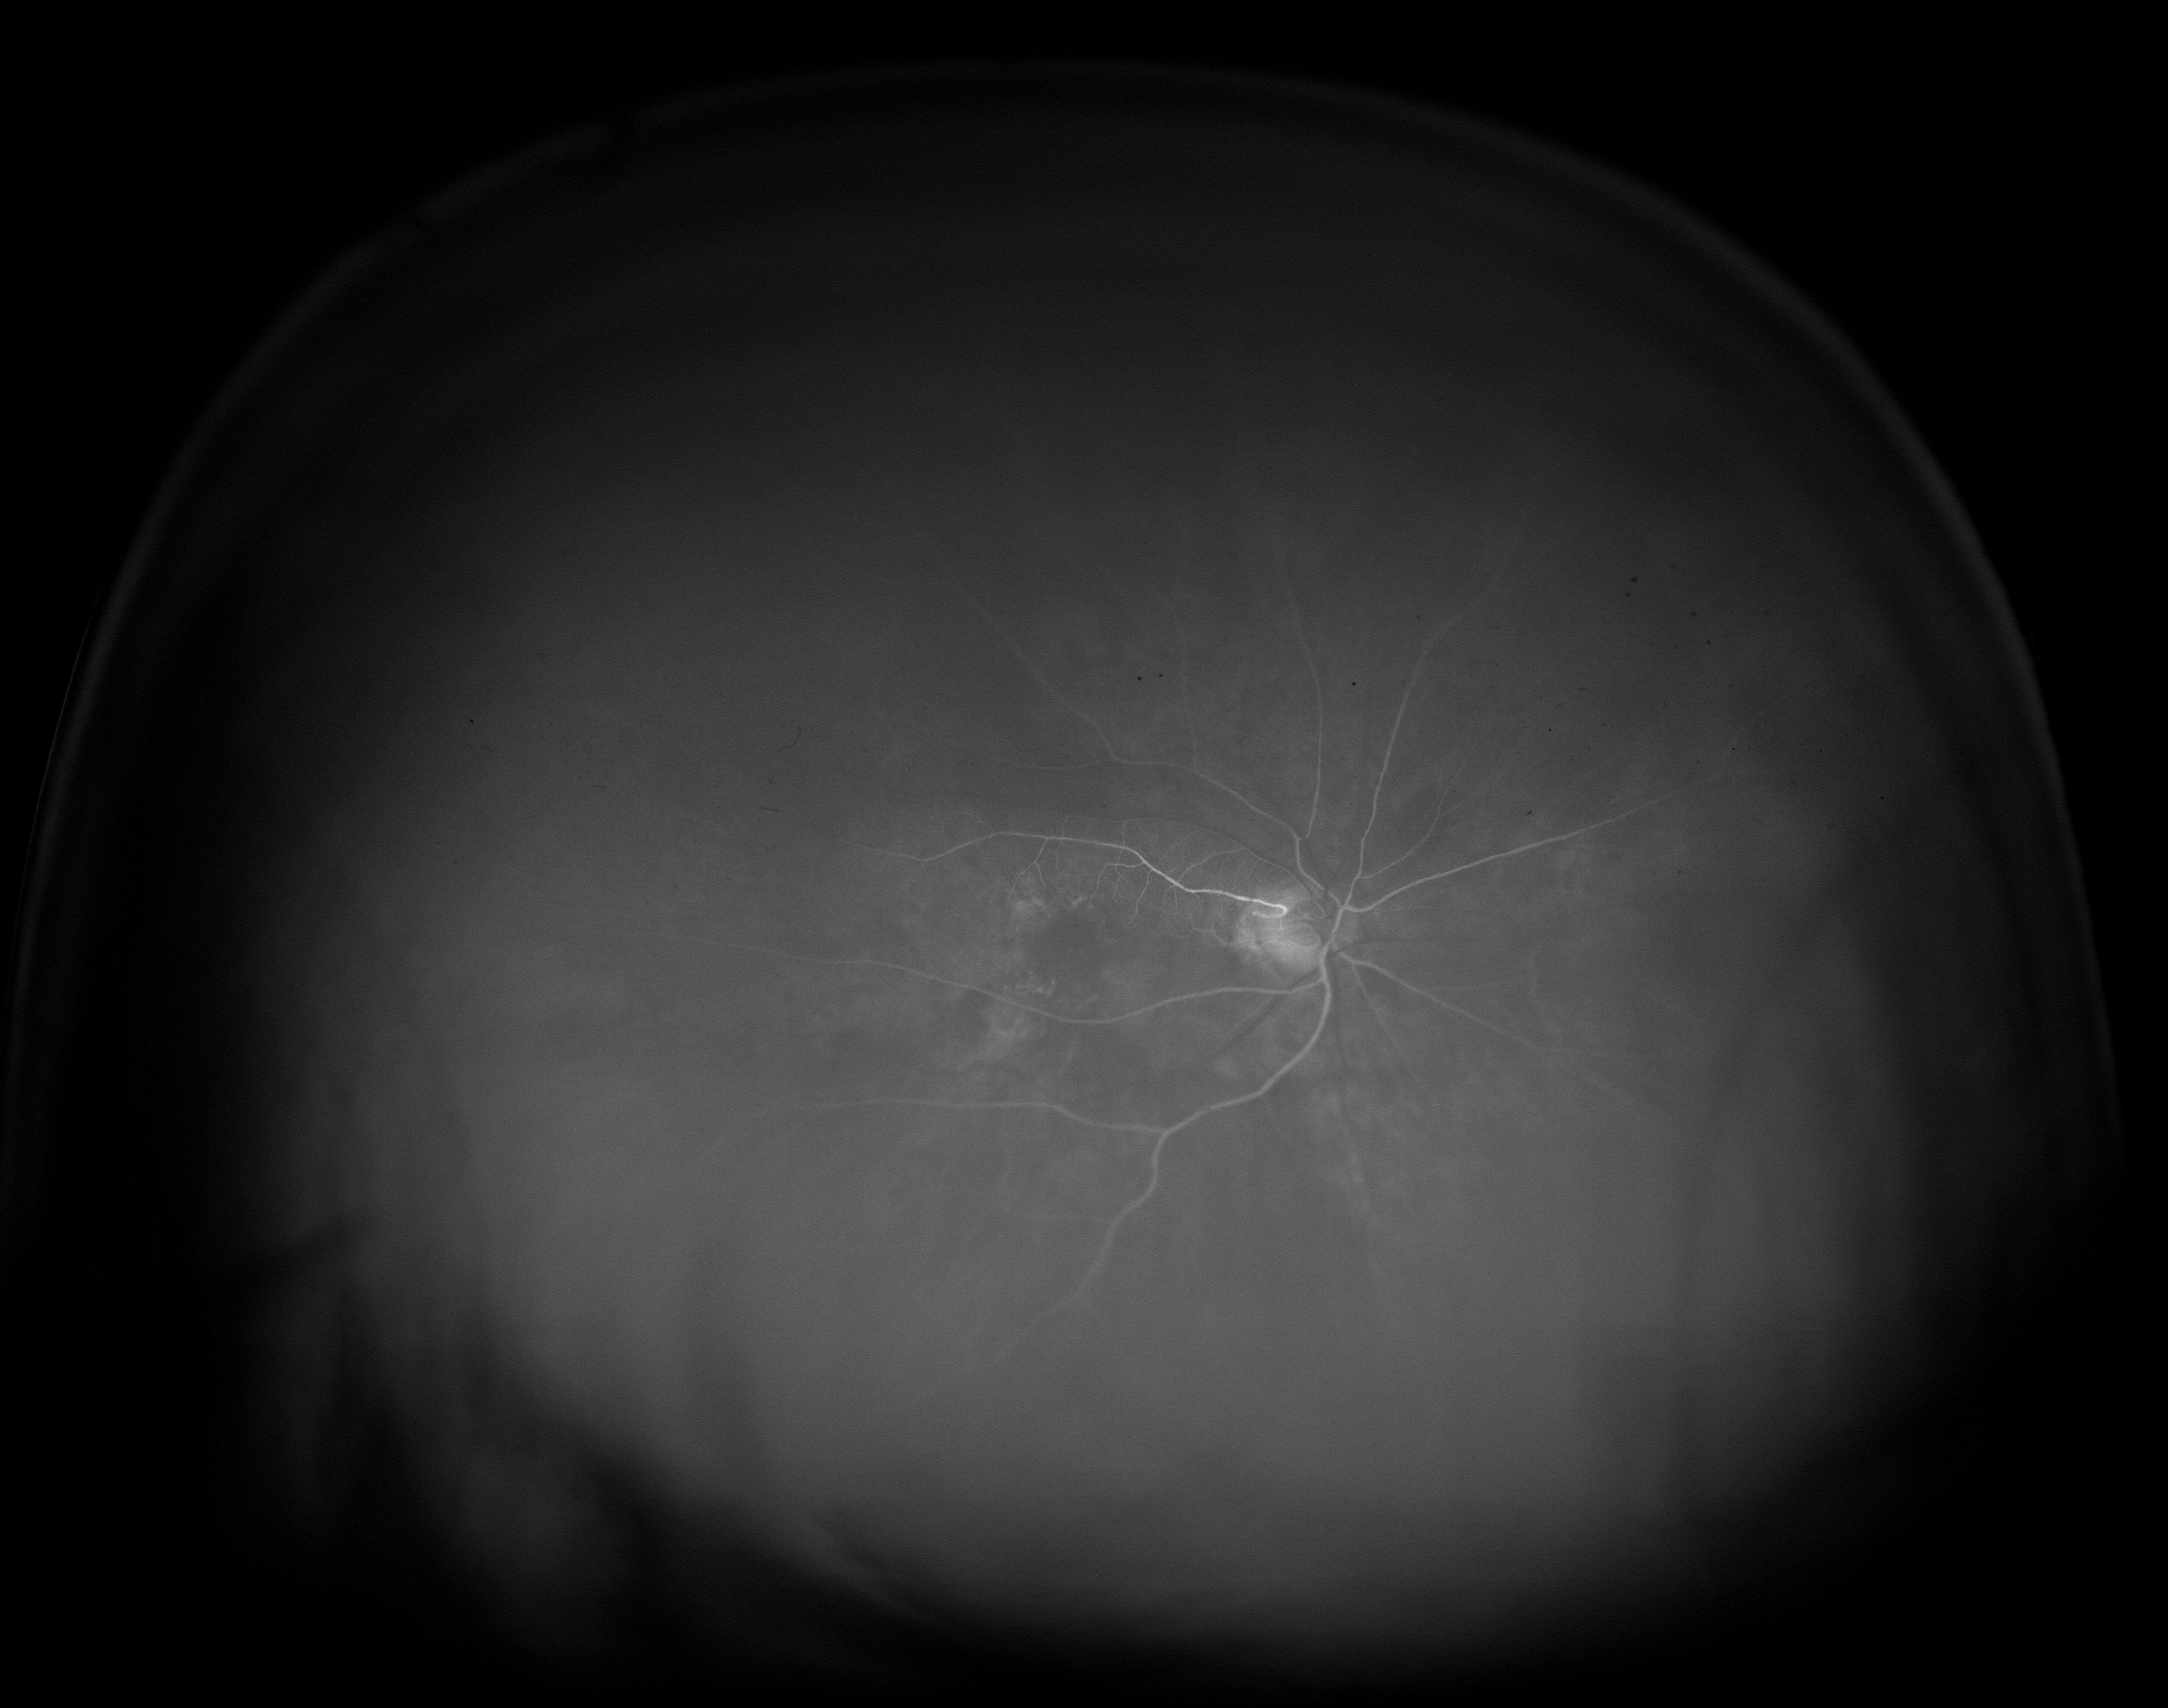
\includegraphics[width=1\textwidth]{./Figures/AF1.png}
        \caption{Fase arterial}
        \label{fig:af1}
    \end{subfigure}
	\begin{subfigure}[b]{0.23\textwidth}
        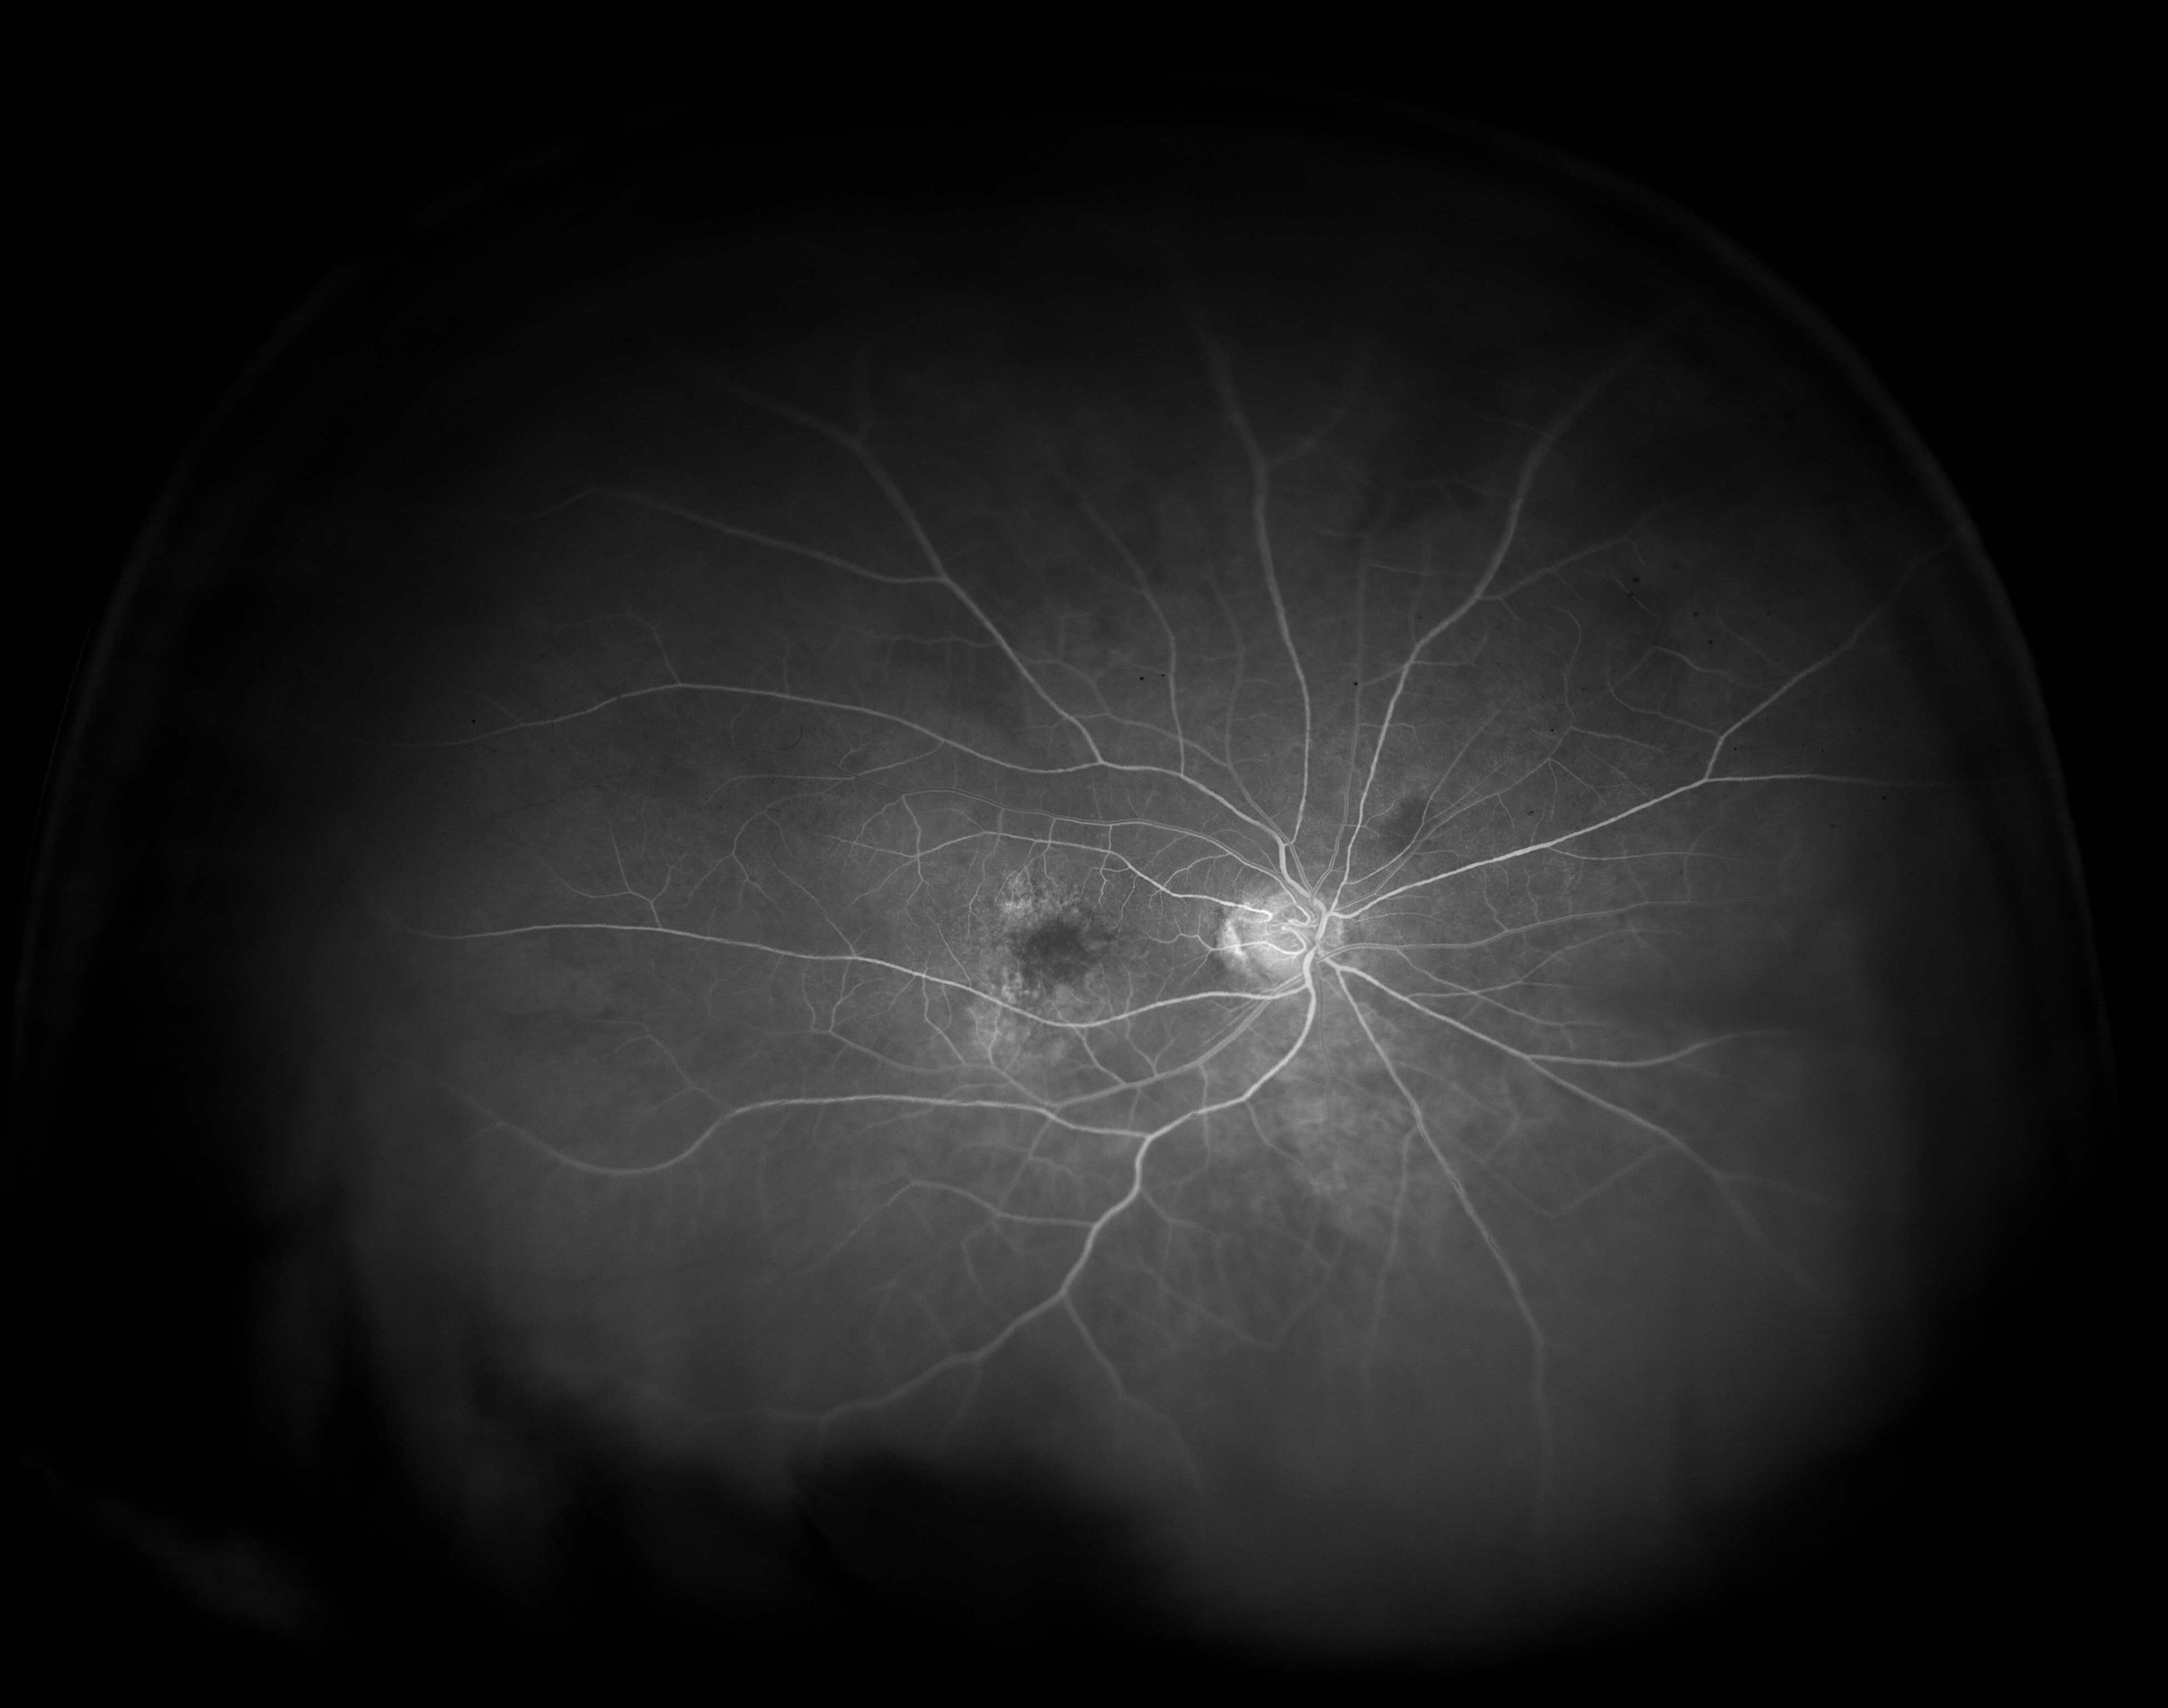
\includegraphics[width=1\textwidth]{./Figures/AF2.png}
        \caption{Fase arteriovenosa}
        \label{fig:af2}
    \end{subfigure}
	\begin{subfigure}[b]{0.23\textwidth}
        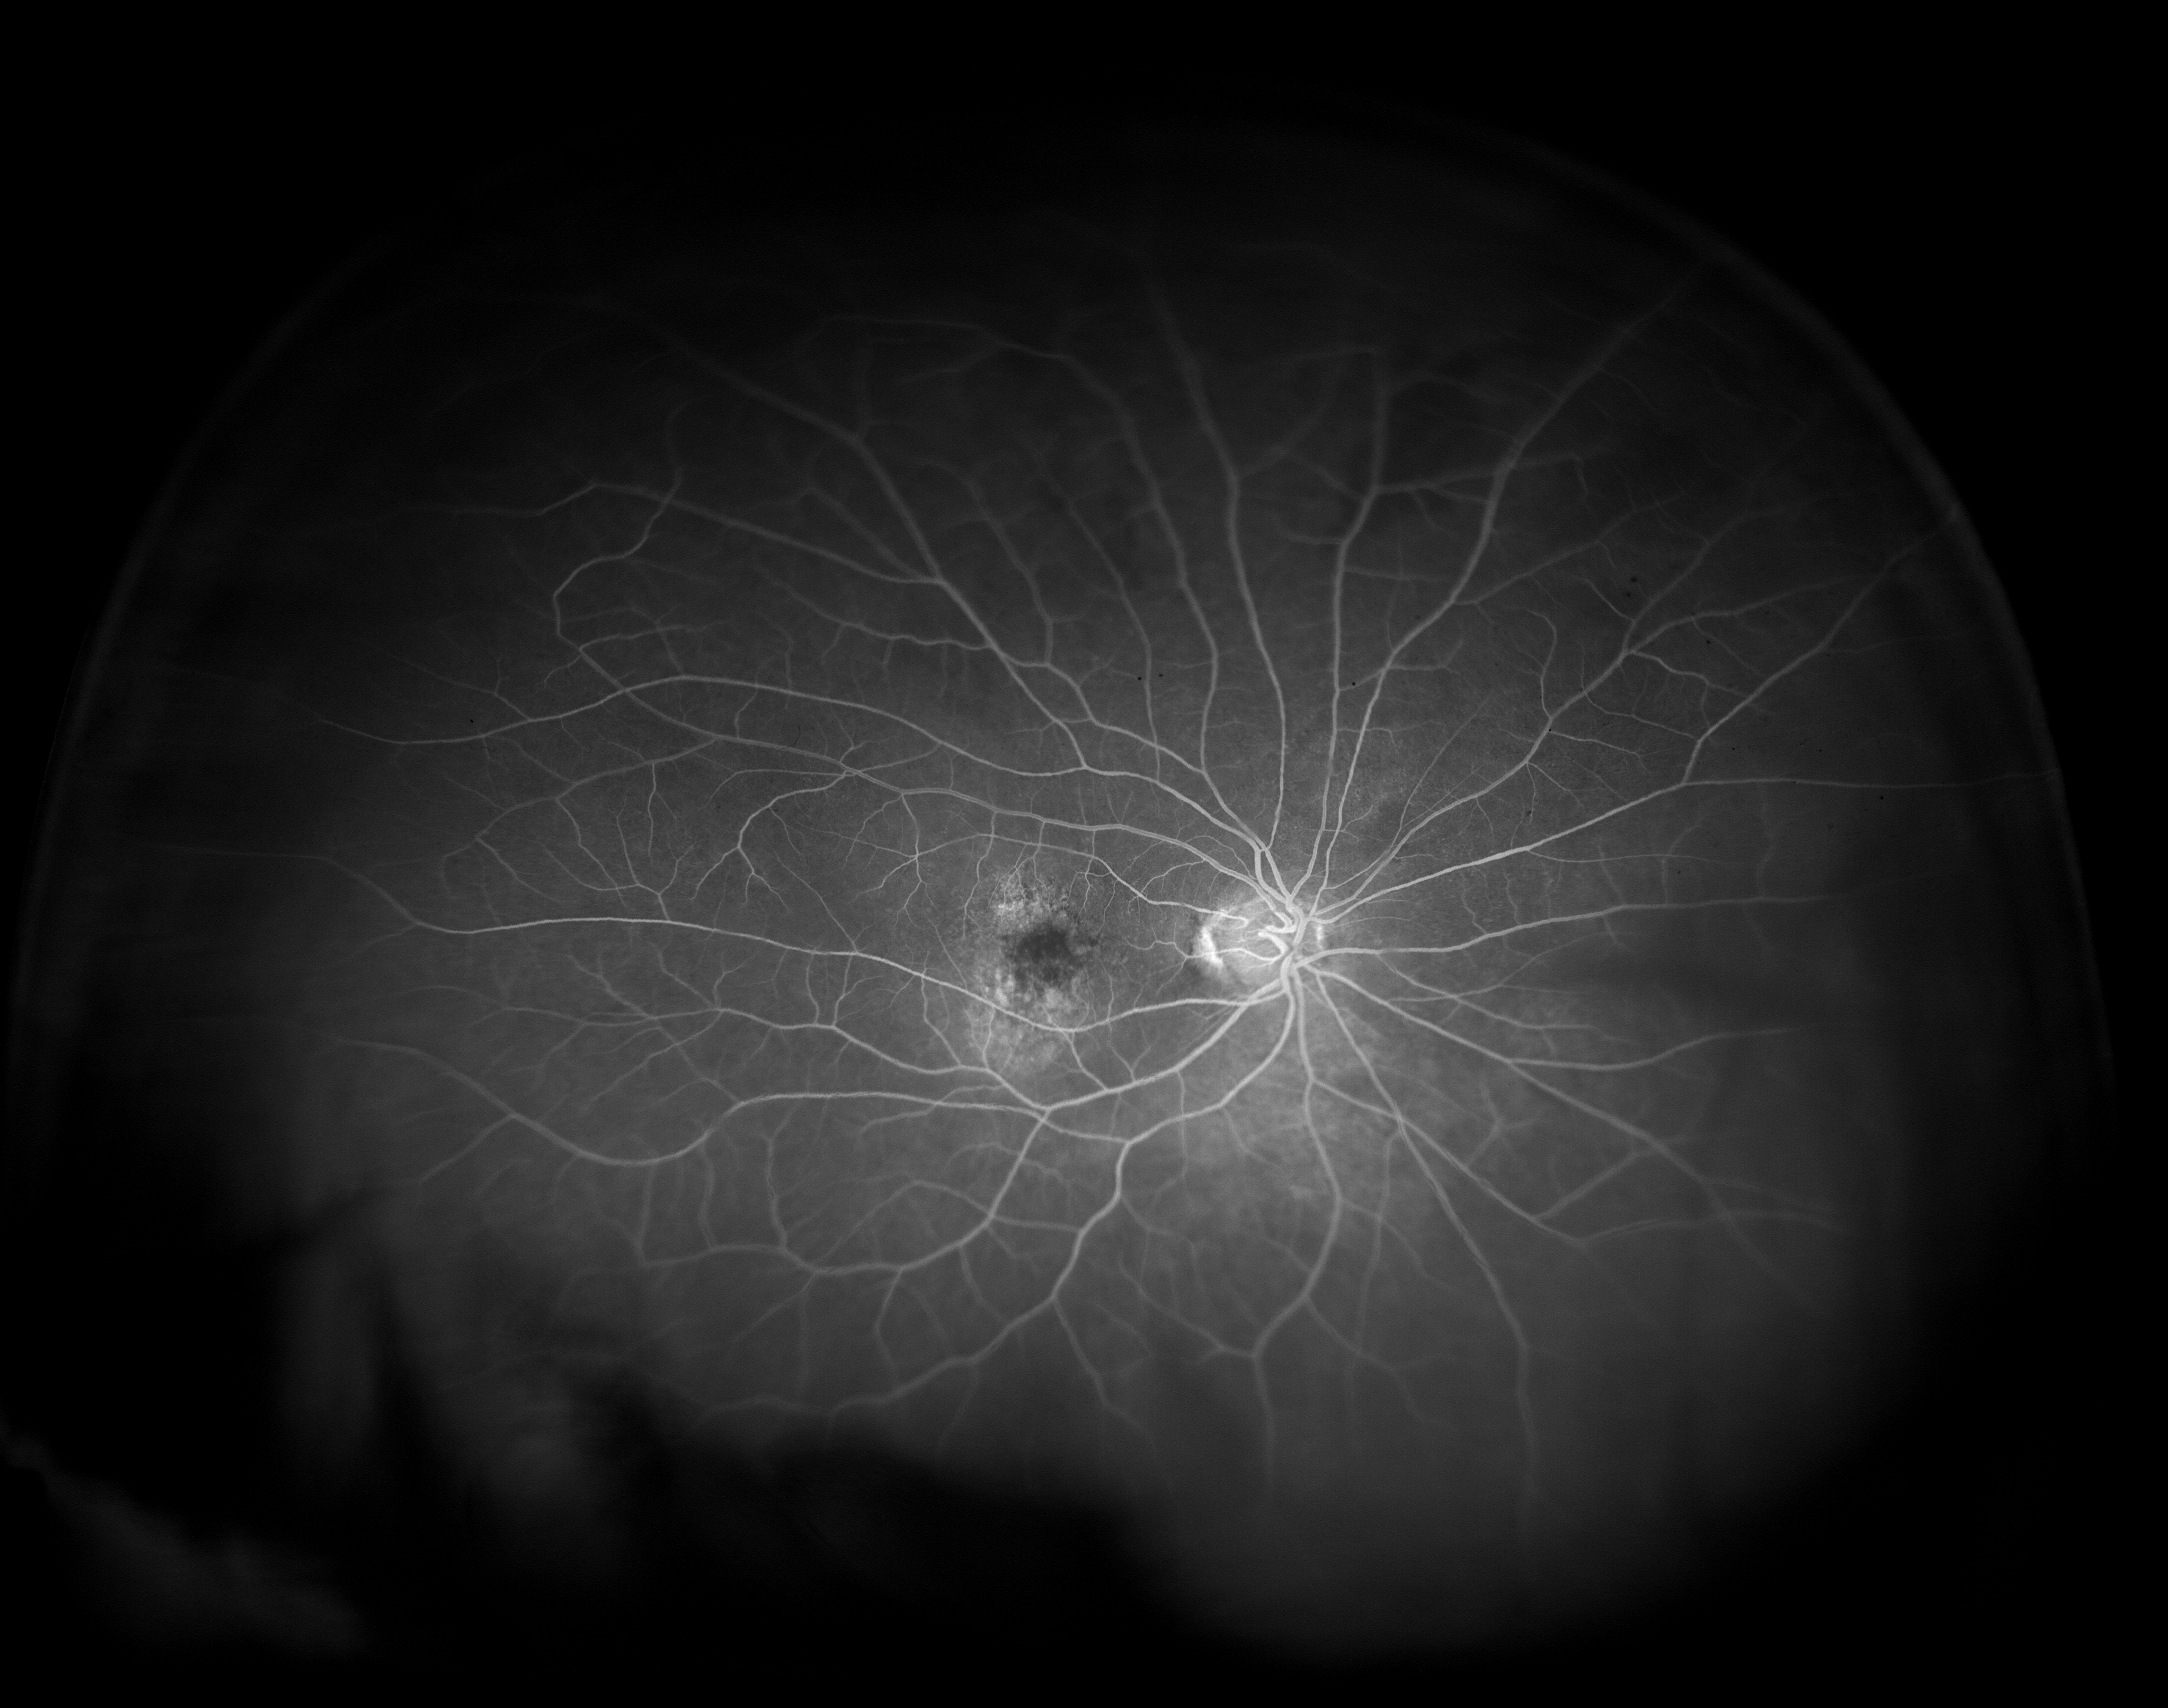
\includegraphics[width=1\textwidth]{./Figures/AF3.png}
        \caption{Fase venosa}
        \label{fig:af3}
    \end{subfigure}
    	\begin{subfigure}[b]{0.23\textwidth}
        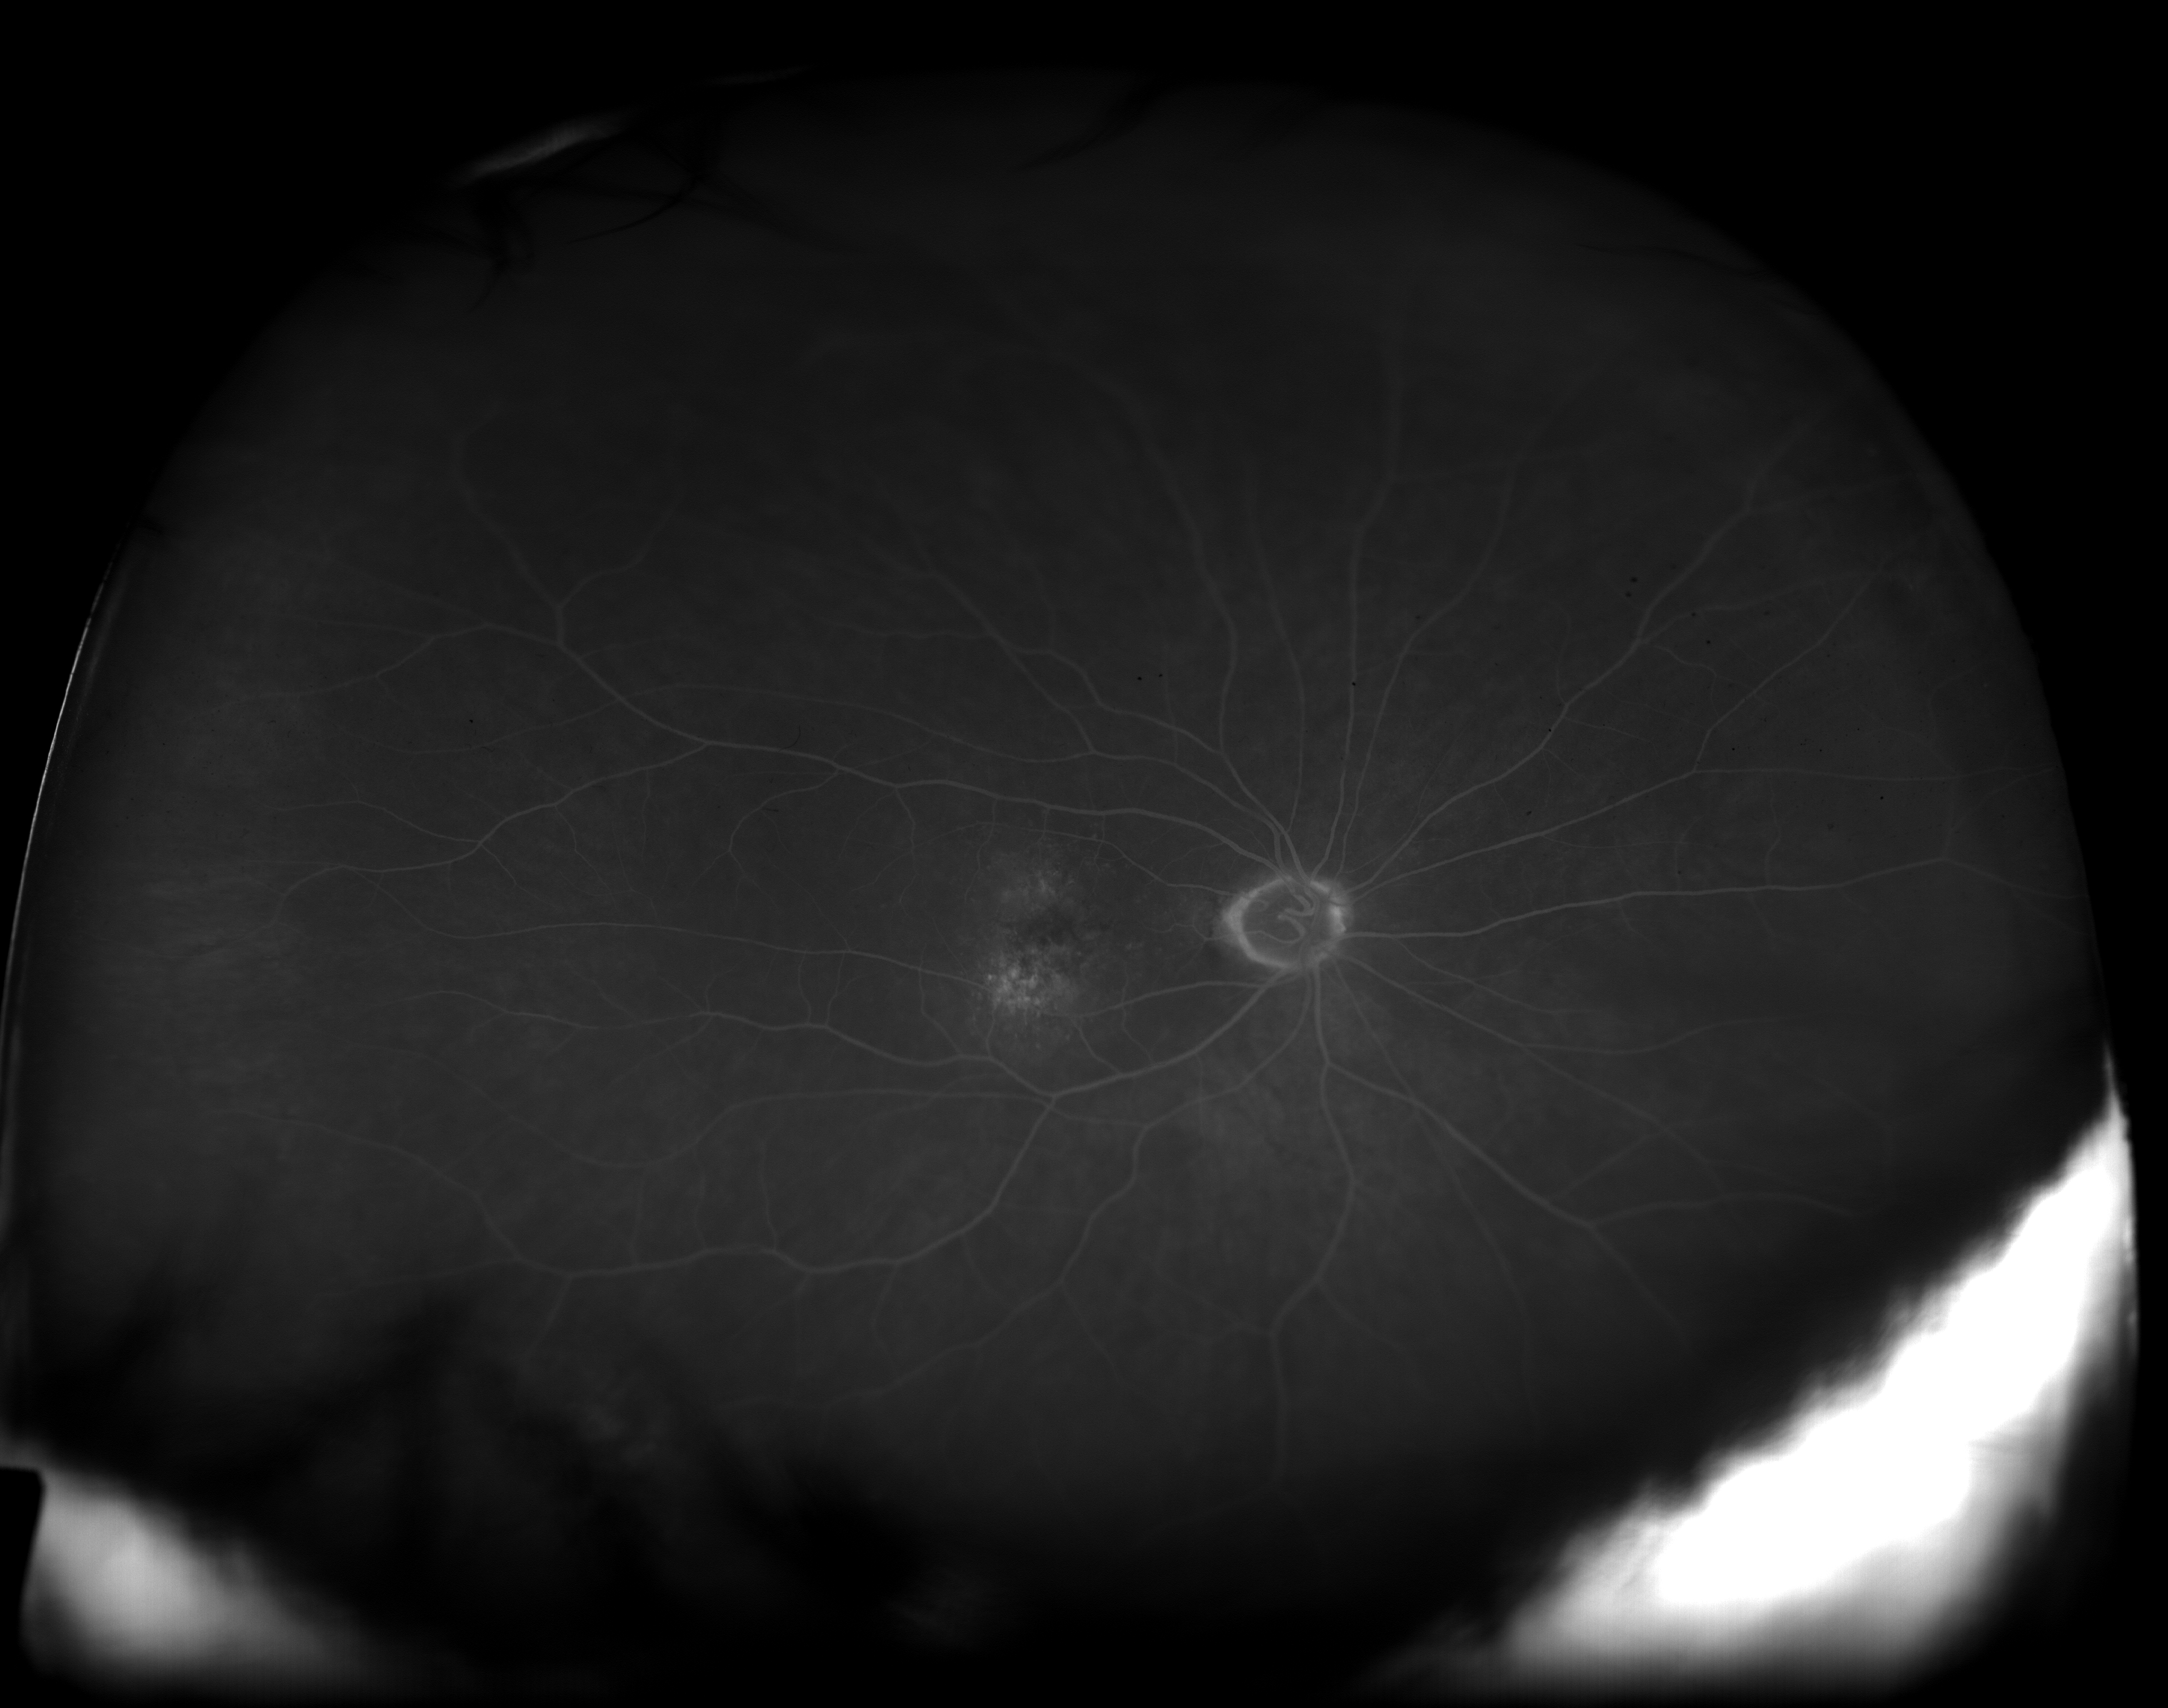
\includegraphics[width=1\textwidth]{./Figures/AF4.png}
        \caption{Fase de eliminación}
        \label{fig:af4}
    \end{subfigure}
	\label{fig:retina}
	\caption{Angiograf\'ia con fluoresc\'ina}
\end{figure}


\begin{figure}[H]
\centering
\includegraphics[width=0.9\textwidth]{./Figures/FA_estrucure.pdf}
\label{fig:lightfilter}
\caption{ Estructura anat\'omicas}
\end{figure}

\begin{figure}[H]
\centering
\includegraphics[width=0.9\textwidth]{./Figures/edemaMacularFA.pdf}
\label{fig:lightfilter}
\caption{ Edema macular}
\end{figure}


\begin{figure}[H]
\centering
\includegraphics[width=0.9\textwidth]{./Figures/retinopatiaFA.pdf}
\label{fig:lightfilter}
\caption{ Retinopatia diabetica}
\end{figure}



\subsubsection{AF para detecci\'on enfermedades }

explicar en qué contextos se las usan, para el diagnóstico de cuáles enfermedades, y qué cosas se ven en ellas.

MALARIA CEREBRAL
Los Intravascular filling defects (IVFD) son características de  MR que pueden ser observadas en imágenes de  angiografías de fluorescencia (AF) .IVFD puede representar secuencias de parásitos eritrocitos en la microvasculatura. Sequestration es la característica patológica de la malaria cerebral , pero hasta ahora , sólo ha sido posible cuantificar histopatológicamente en el post mortem . IVFD puede ser visto en pequeñas y largas vénulas arteriolas y los capilares , pero parecen ser más prominente en las vénulas. Sequestration del cerebro y la retina es siempre visto en casos fatales de MC con RM, y la apariencia de la histopatología es similar en IVFD. Además, IVFD a menudo resuelve el dia despues del tratamiento con medicamentos contra la malaria. Esto es consonancia con  la resolución de sequestration y la recuperación clínica. Es plausible que  IVFD representa proceso patológico fundamental, y esta lesión merece una mayor investigación. \cite{zhao2015automated}

IMAGEN

\textbf{Edema Macular Diabético}

La angiografía de fluorescencia es una poderosa herramienta para la captura de imagenes y evaluación del edema macular diabético (EMD). donde el tinte fluorescente se acumula en las áreas enfermas.
El EMD es un proceso patológico que consiste en la anormal permeabilidad de la retina que resulta en la fuga y acumulación de fluidos en la capa de la retina del ojo. Es definido como la presencia de engrosamiento de la retina que involucra la mácula, definida como el área a 2 discos ópticos de distancia desde el centro de la visión (ej. fóvea ). El resultado es la visión borrosa en el paciente y puede conducir a la deficiencia visual en etapas adelantadas si no se trata. \cite{el2011segmentation}

IMAGEN

El Edema Macular Diab\'etico, en particular, es un gran contribuyente a la p\'erdida de la visi\'on  entre pacientes con Retinopat\'ia Diab\'etica. Hace m\'as de 25 a\~nos, el Early Treatment of Diabetic Retinopathy Study (ETDRS) estableci\'o gu\'ias para identificar los edemas maculares cl\'inicamente significativos y prob\'o que el tratamiento con fotocoagulaci\'on con laser focal decrementa el riesgo de perdida moderada de la visi\'on, incrementa las posibilidades de ganancia visual moderada y reduce el engrosamiento retinal. \textbf{While ETDRS remains the seminal study on DMO, additional awareness of diabetic pathology,} el advenimiento de la nueva farmacolog\'ia y las mejoras en la tecnolog\'ia de captura de im\'agenes de la retina nos han permitido expandir nuestro entendimiento y tratamiento del edema macular diab\'etico.
Hace tiempo se ha hipotetizado que los cambios isqu\'emios y las patolog\'ias microvasculares  juegan un papel en el desarrollo del Edema Macular Diab\'etico. En la Retinopat\'ia Diab\'etica, la isquemia estimula la producci\'on de factor de crecimiento vascular endotelial(VEGF, por sus siglas en ingl\'es), lo que puedo conducir al quiebre de las barreras sangre-retina, y puede causar Edema Macular Diab\'etico por incremento de la permeabilidad de los vasos sangu\'ineos. Las drogas Anti-VEGF han probado eficacia en el tratamiento del Edema Macular Diab\'etico, incluso en los casos que no responden a la fotooagulaci\'on por laser. El \'exito de la terapia anti-VEGF da sustento a la idea de que la isquemia retinal y el Edema Macular Diab\'etico est\'an asociados, pero la captura de im\'agenes de retinal tradicional dificulta el estudio de esta asociaci\'on.
La isquemia retinal se caracteriza mejor utilizando angiograf\'ias fluorescentes(FA). Las FA tradicionales emplean fotograf\'ia retinal que es capaz de ver aproximadamente 30\degree de la retina por im\'agen. El ETDRS desarrollo el protocolo \textbf{the seven-standard fields (7SF)} en donde 7 \'areas de la retina fotografiadas son combinadas para dar una visualizaci\'on cercana a 75\degree. Con el advenimiento de las angiograf\'ias fluorescentes de ultra campo de visi\'on (UWFA), as\'i como de los sistemas de captura Optos 200Tx, es ahora posible ver 200\degree de la retina en una sola fotograf\'ia. Los estudios a peque\~na escala iniciales mostraron que las UWFA son m\'as \'utiles en la detecci\'on de la no perfusi\'on de capilares en pacientes con Edema Macular Diab\'etico que otros m\'etodos con campos de visi\'n m\'as limitados en la captura de im\'agen.\citep{wessel2012peripheral}

	\subsection{Herramientas computacionales para an\'alisis de agiograf\'ias con fluoresce\'ina}



\section{Segmentaci\'on de vasos sangu\'ineos en FA}

	\subsection{Necesidad}
	

	\subsection{M\'etodos existentes}



	\subsubsection{Supervisados}

En los m\'etodos supervisados, la regla para extracci\'on de vasos es aprendida por un algoritmo en base a un conjunto de im\'agenes de referencia manualmente procesadas y segmentadas generalmente llamadas estandar de oro. Estas estructuras vasculares en dichas im\'agenes son marcadas con presici\'on por un oftalmologo. Sin embargo, como menciona Hoover et al. \cite{hoover2000locating} existe un desacuerdo significativo en la identificaci\'on de vasos incluso entre observadores expertos. En un m\'etodo supervisado, el criterio de clasificaci\'on es determinado por los datos de referencia basados en las caracter\'isticas seleccionadas. Por lo tanto el pre-requisitos es la disponibilidad de im\'agenes de referencias clasificadas, las cuales muchas veces no est\'an disponibles en aplicaciones de la vida real. Como estos m\'etodos est\'an dise\~nados basados en datos pre-clasificados, su desempeño es generalmente mejor que aquellos que no son supervisados y pueden producir muy buenos resultados para im\'agenes "saludables" de la retina.

	\subsubsection{No supervisados}


Los enfoques basados en clasificaci\'on no superviada intentan encontrar los patrones inherentes a los vasos sang\'ineos de las im\'agenes de la retina que pueden ser utilizados para determinar si un pixel en particular pertenece o no a un vaso. Los datos de referencia no contribuyen directamente al dise\~no del algoritmo en estos enfoques.

En general, existen tres principales desafios que deben abordarse en el automatizado de la segmentación de vasos de la retina :
\begin{enumerate}
\item La calidad de imagen es a menudo un problema de interés para el desarrollo de la segmentación automatizada. Técnicas de segmentación existentes todavía se enfrentan a desafíos en la segmentación de toda la vasculatura con precisión , debido al poco contraste, fondos no homogéneos y la presencia de ruido durante la adquisición de imagen.
\item La complejidad de la estructura vascular (por ejemplo, múltiples escalas y orientaciones), el alto grado de variación anatómica a través de la población y la complejidad de los tejidos / órganos de alrededores
, plantean desafíos significativos en segmentación de los vasos. El realce de los vasos es
una forma efectiva para facilitar la segmentación:  pero comúnmente usar filtros de realce no es en términos de rendimiento.
\item Un eficiente y robusto modelo de segmentación  es deseable. Se ha vuelto muy difícil
para elegir un modelo óptimo, o para identificar un único conjunto de parámetros óptimos para un método de segmentación en particular que trabaje a través de una variedad de datos.\cite{zhao2015retinal}
\end{enumerate}



\subsubsection{métodos de segmentación en FA}
*****métodos de segmentación en FA******
